\section{Designentwicklung}

\subsection {Paperprototyp}

Mit der Festlegung des Szenarios sind die ersten Ansätze entstanden.
Für das erste Design wurde die Methode des Paper Prototyp genutzt. 
Dabei handelt es um eine handgezeichnete Skizze, die genutzt wird, um erste Ideen visuell darzustellen.  
Hierbei können einfache Prozesse, Umrisse und Komponenten frei eingezeichnet werden.
 Im Design Thinking wird diese Art des Low-Fidelity-Prototyping gerne eingesetzt da der Prozess schnell und einfach ist, um die Grundkonzepte festzuhalten. 

\begin{figure} [ht]
\begin{center}
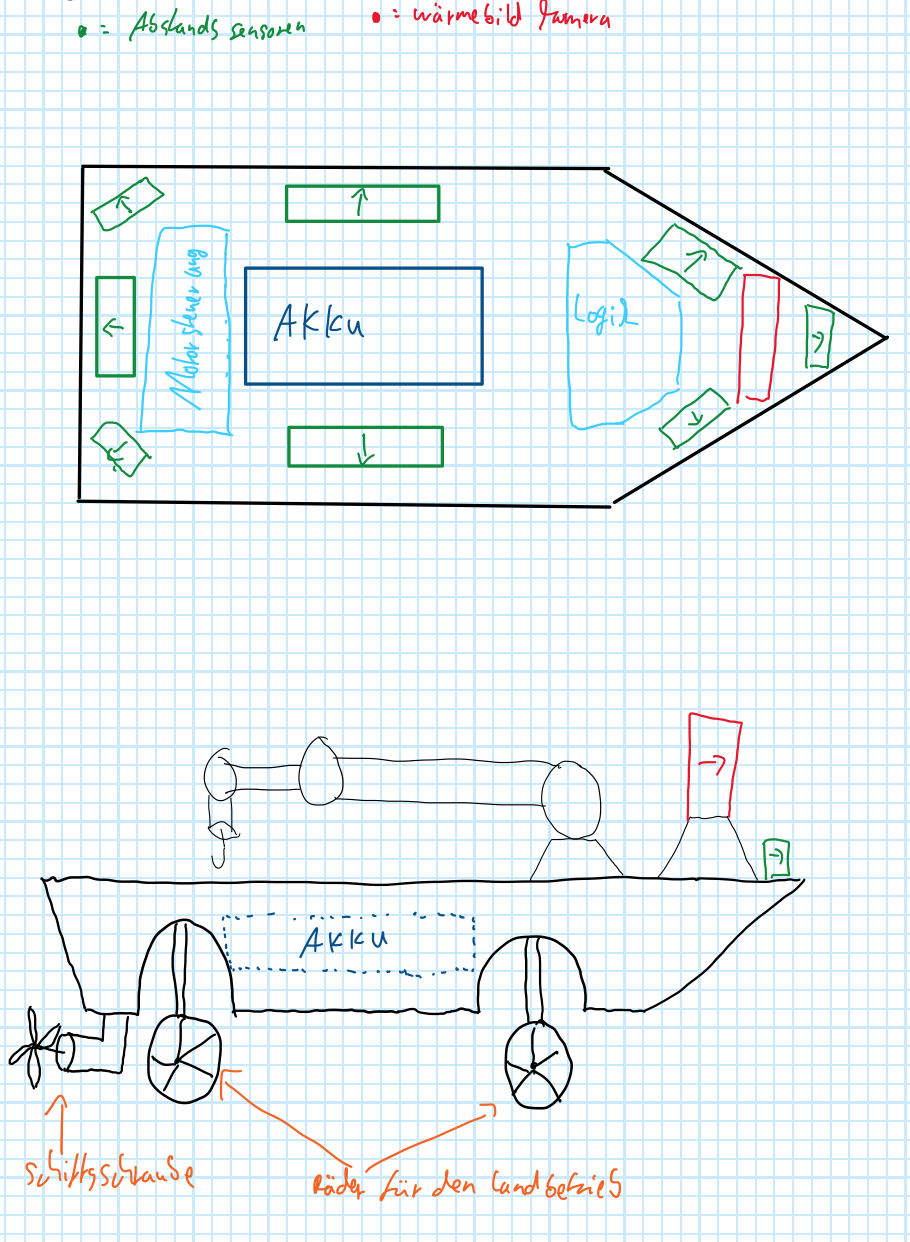
\includegraphics [width = 0.4\textwidth] {PaperPrototype.PNG}
\caption {Erster Paper Prototyp}
\end {center}
\end {figure}

Auf der ersten Paper Prototyp Skizze sind zwei Perspektiven des Roboters dargestellt. 
Die obere Perspektive zeigt die Ansicht von Oben auf den Roboter.
Die untere zeigt die seitliche Perspektive. Auf den ersten Blick ist zu erkennen, dass es sich um ein Hybriden Roboter handelt.
Dieser soll durch die Skizze schon zeigen, dass das Fahren auf dem Land und auch auf dem Wasser möglich ist. 
Auffällig ist die spitzzulaufende Form im vorderen Bereich. 
Die Bug-Form ähnelt der eines Boots oder Schiffs. 
Zudem erkennt man im hinteren Bereich, unten angebracht eine Schiffsschraube. 
Für den Landbetrieb sind Räder eingezeichnet. 
Die vier Räder befinden sich im unteren Bereich. 
Der Roboter soll die Möglichkeit haben Hindernisse wegzuräumen und Personen zu helfen. 
Dafür wurde ein Greifarm auf dem Roboter eingezeichnet.  
Dieser Greifarm kann vielseitig eingesetzt werden. 
Auf der Ansicht von Oben sind einige Details skizziert.
 So befinden sich dort insgesamt acht Abstandssensoren in verschiedenen Richtungen. 
Im hinteren Bereich ist die Motorsteuerung eingezeichnet, mittig ein Akku als Energieversorgung und vorne eine Logikkomponente.
Im vordersten Bereich ist eine Wärmebildkamera eingeplant für den Einsatz in Hitzebereichen. 
Die Skizze zeigt somit die wichtigsten Komponenten und die Grundidee.
Die Veranschaulichung stellt dar wie der Landbetrieb und Wasserbetrieb grob funktionieren soll. 
Zudem wird die Idee eines multifunktionalen Greifarms dargestellt.

\subsection {Erste 3D-Modellierung}

\begin{figure} [ht]
\begin{center}
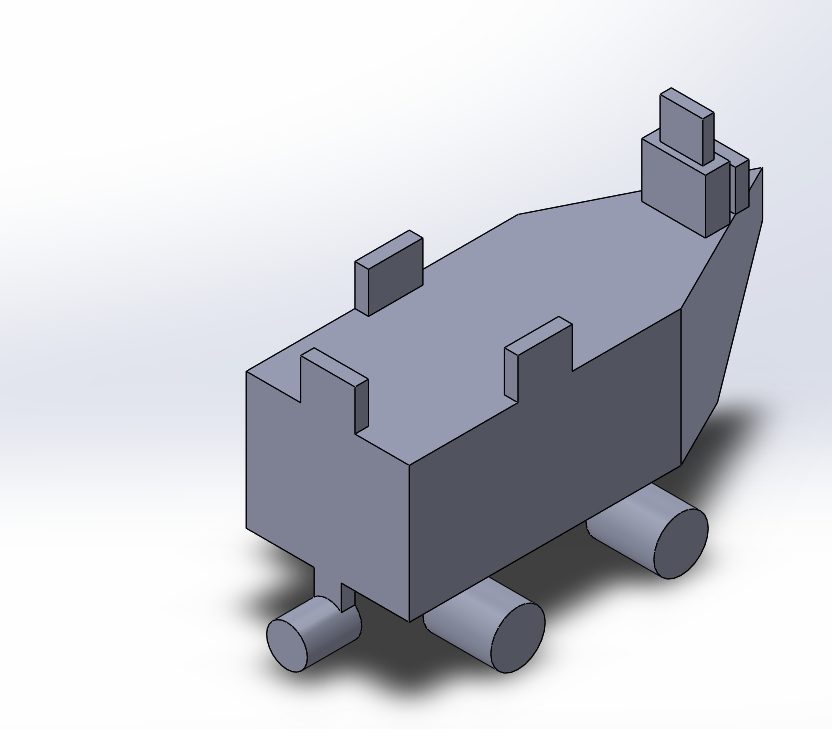
\includegraphics [width = 0.4\textwidth] {CadV1.PNG}
\caption {Erstes CAD-Modell}
\end {center}
\end {figure}

Im Folgenden ein erstes Rendering des Prototyps in SolidWorks erstellt. Dabei handelt es um ein CAD Programm welches rechnerunterstützte Konstruieren ermöglicht. Das Modell wird 3-dimensional dargestellt. So ist ein räumliches Verständnis möglich und die grobe Form wird erkennbar. Auf dem Rendering zeigt sich die Bug-Form vorne, unten die vier Räder und hinten die Schiffsschraube. Im oberen Bereich sind erste Sensoren angebracht, sowie im vorderen Bereich eine Kamera. Der Greifarm wie er auf der Skizze zu sehen ist, ist nicht im Rendering. Das 3D-Rendering stellt die grobe Bauweise und Form vereinfacht dar.

\subsection {Reale Beispiele}

\begin{figure} [ht]
\begin{center}
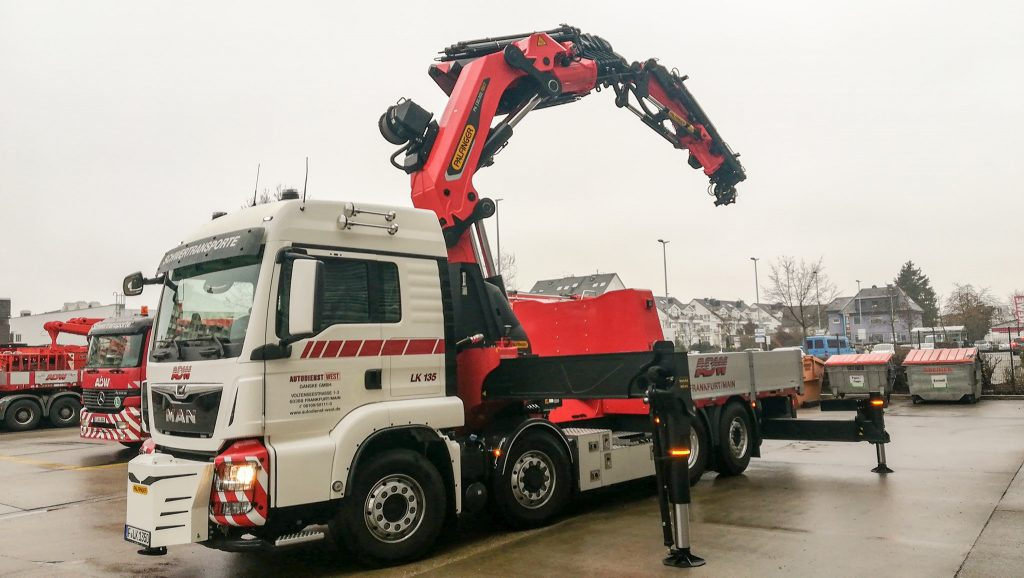
\includegraphics [width = 0.25\textwidth] {Ladekran.jpg}
\caption {Ladekran}
\end {center}
\end {figure}

\begin{figure} [ht]
\begin{center}
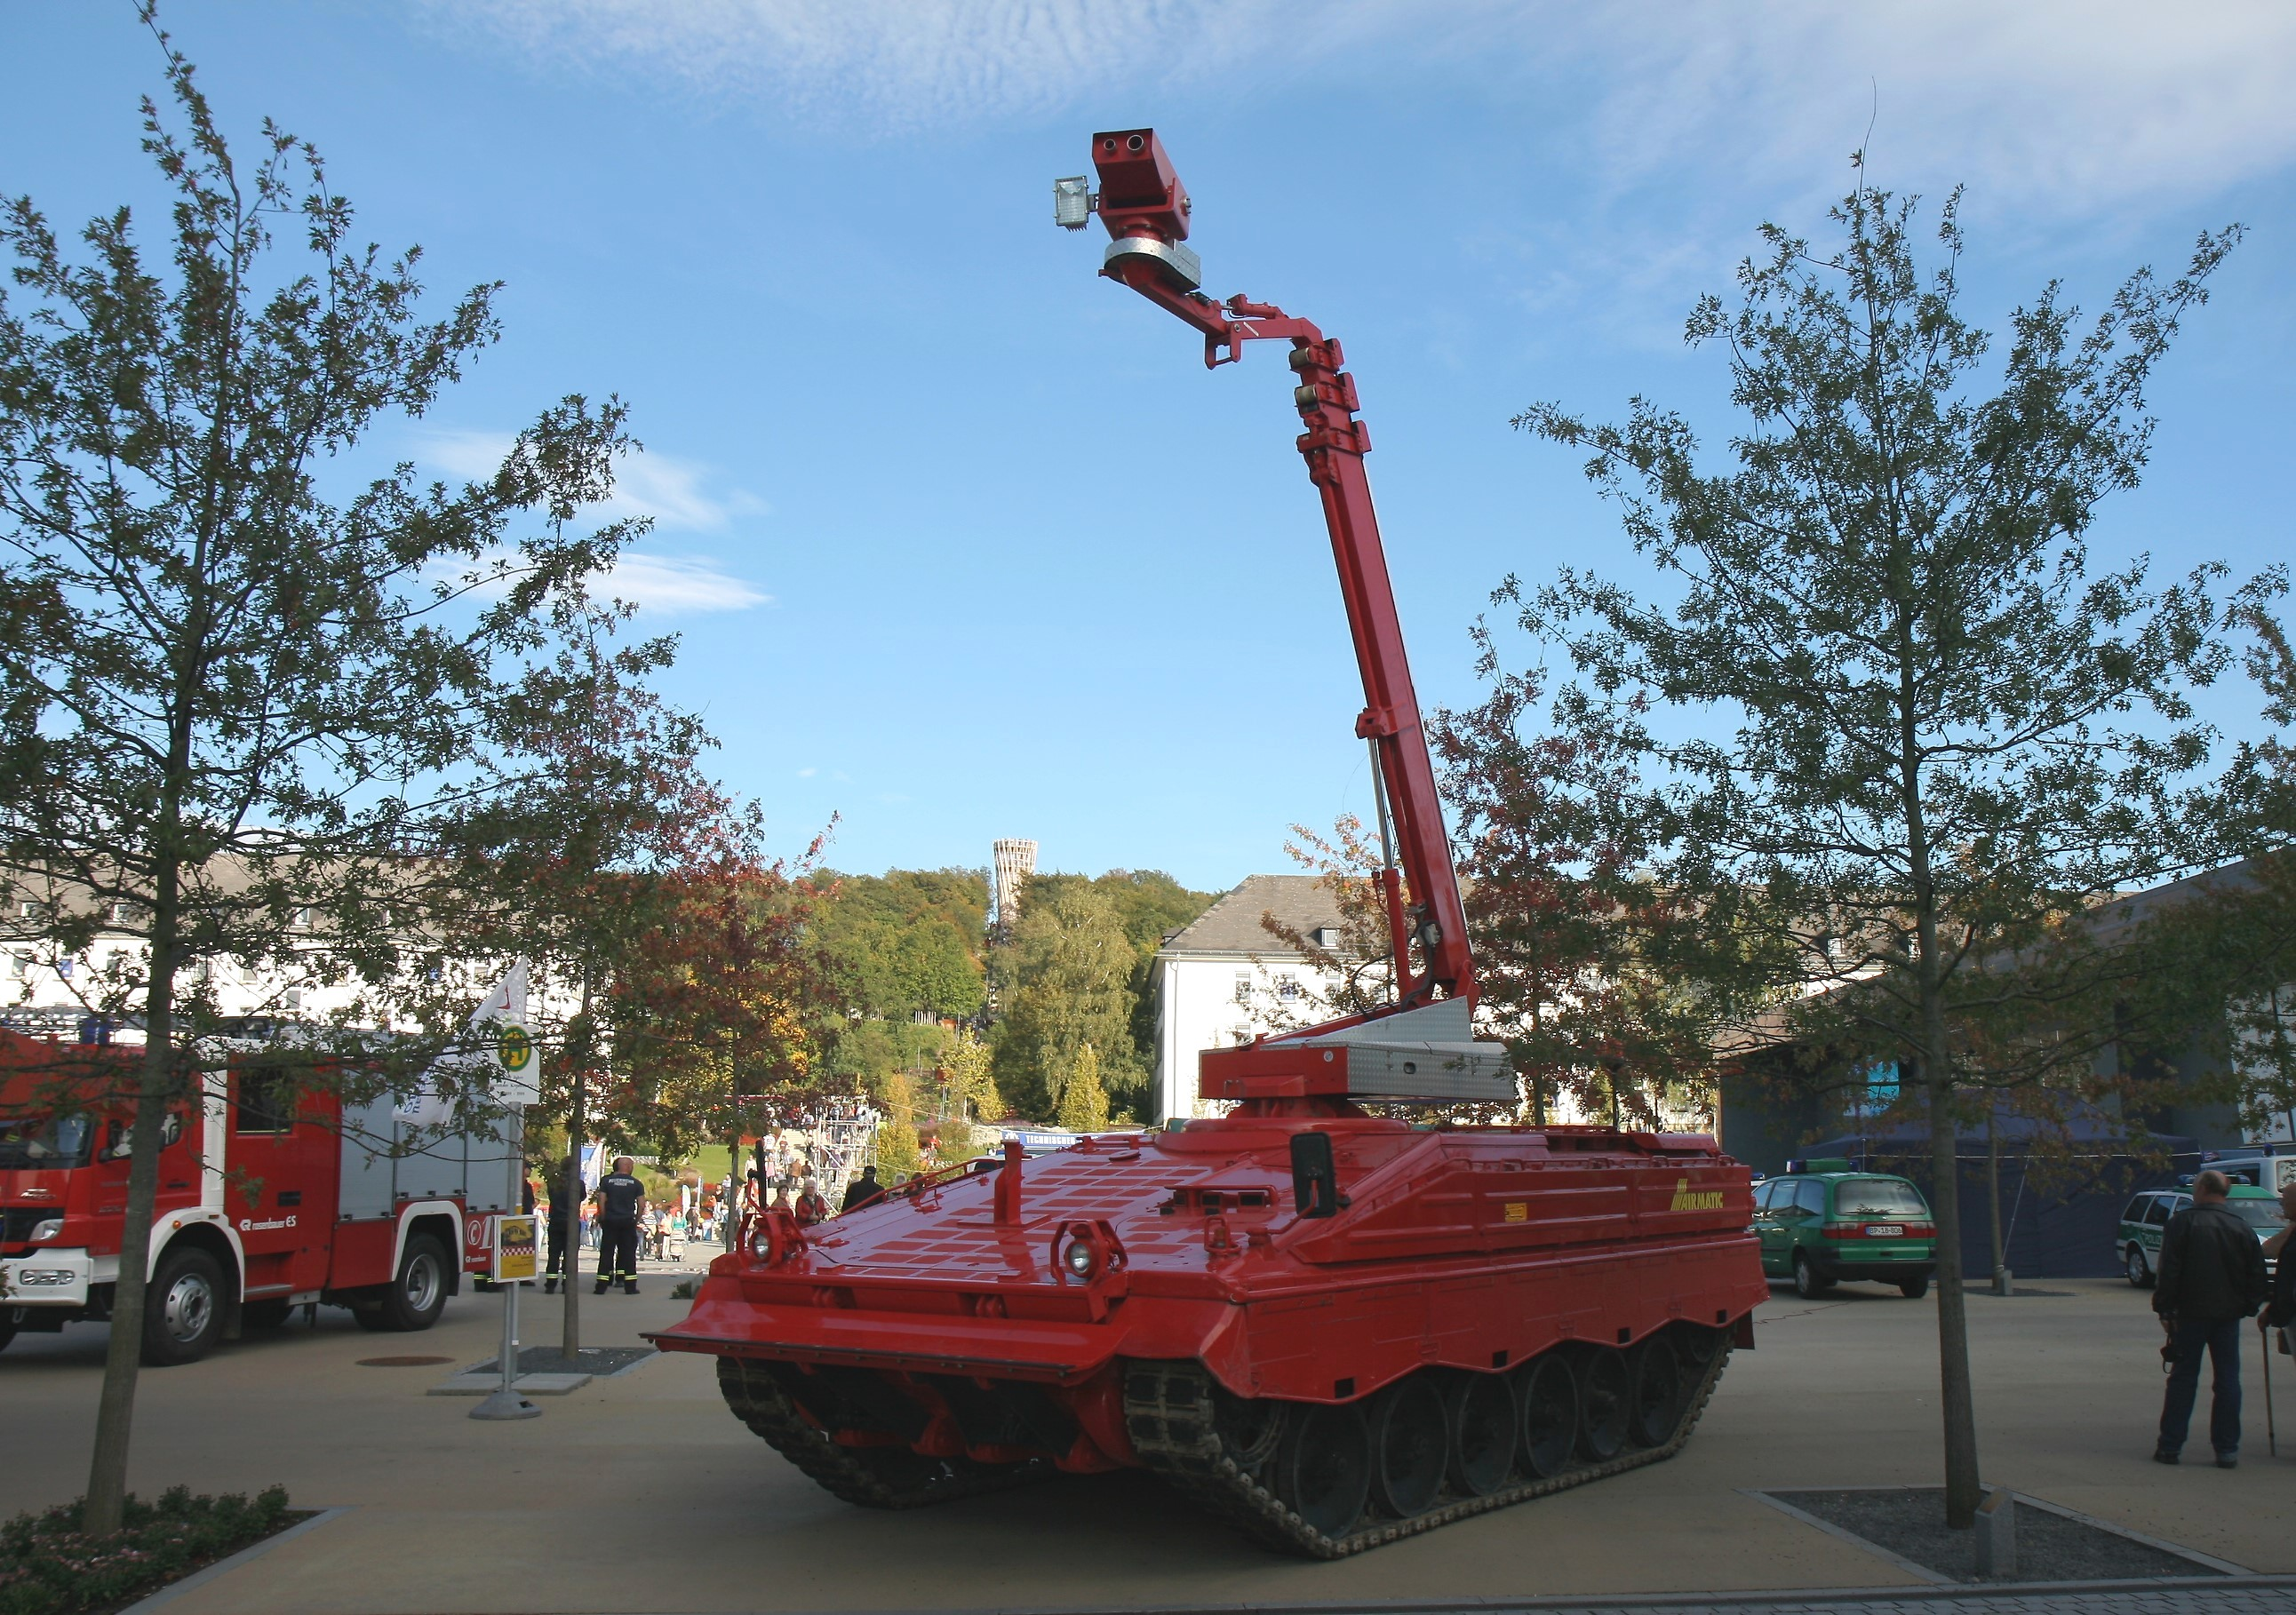
\includegraphics [width = 0.25\textwidth] {Loeschpanzer.jpg}
\caption {Löschpanzer}
\end {center}
\end {figure}

\begin{figure} [ht]
\begin{center}
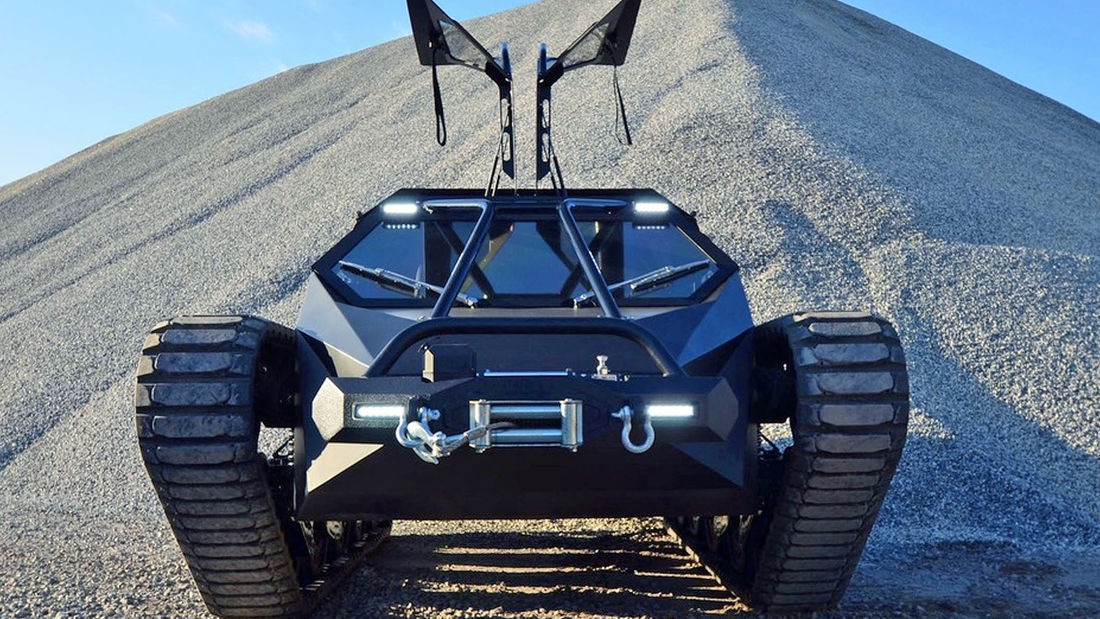
\includegraphics [width = 0.25\textwidth]{Kettenfahrzeug.jpg}
\caption {Kettenfahrzeug}
\end {center}
\end {figure}

Im Verlauf des Projekts wurde das Szenario genauer untersucht und analysiert. 
Die Use Case Anforderungen wurden definiert. Das Design ist mit den Anforderungen gewachsen und hat sich teilweise verändert.
Da es sich um ein echtes Szenario halten könnte, wurde der Blick auf Beispiele aus dem echten Leben gerichtet. 
Die Recherche zeigte das unsere Ideen schon teils real umgesetzt wurden. 
So gibt es LKWs mit Ladekränen die auch schwere Lasten heben können. 
Dabei ist der Vorteil, dass der Kran bzw. Greifarm durch den LKW flexibel überall hingefahren werden kann, je nach Einsatzgebiet. 
Die Hydraulik ermöglicht dem Greifarm einen großen Radius abzudecken und verschiedene Höhen und Winkel anzusteuern.
Des Weiteren ergab die Recherche das die Feuerwehr teils Löschpanzer nutzt, welche auf Ketten fahren und aus einem feuerfesten Material sind. 
Die Recherche ergab das es bestimmt Kettenantriebe gibt, die auch für höhere Steigungen geeignet sind.
Zudem eignen sich Ketten wie an dem Löschpanzer auch für höhere Temperaturen da diese nicht schmelzen.
Der Ausblick zeigte das bereits echte Fahrzeuge existieren und die Komponenten auf einen neuen Rescue Roboter angewendet werden können. 

\subsection {Prototyp mit Kettenantrieb}

\begin{figure} [ht]
\begin{center}
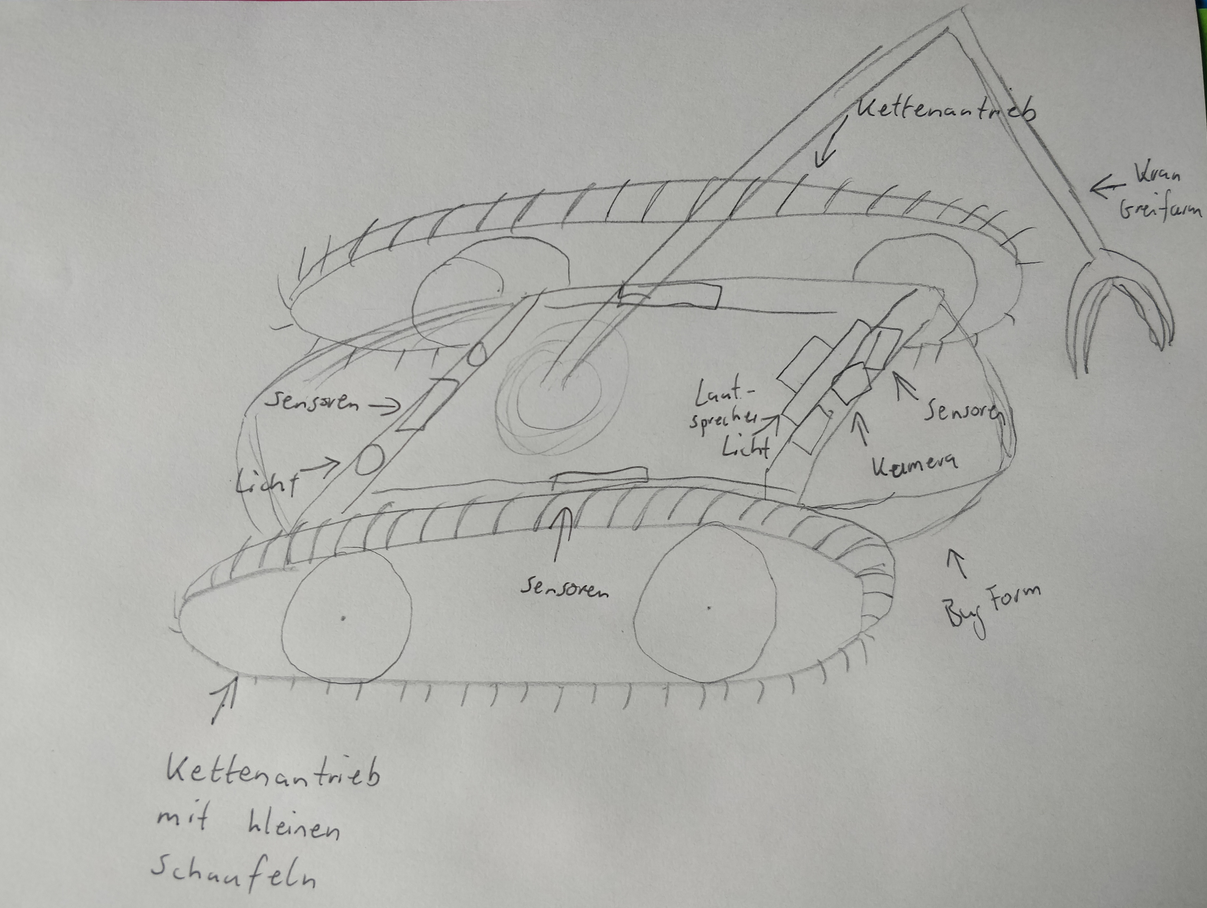
\includegraphics [width = 0.4\textwidth]{PaperPrototype_Ketten.PNG}
\caption {Ein weiterer Paper Protoyp}
\end {center}
\end {figure}

Im weiteren Verlauf erfolgte eine weitere Paper Prototyp Skizze.
In der Recherche ergab sich, dass es für bestimmte Hitze und Feuersituationen spezielle Löschpanzer gibt. 
Die Panzerkettenansatz wurde übernommen. Bei einer erhöhten Temperatur besteht die Gefahr, dass gummierte Reifen schmelzen können und so ein Rettungsvorgang nicht mehr möglich ist.
Um sicher zu sein, wurde das Design des Roboters etwas verändert und statt Rädern folgte ein Kettenantrieb.
Dieser hat zu dem Zeitpunkt einen Kettenantrieb mit kleinen Schaufeln, um sich im Wasser fortzubewegen als temporäre Alternatividee.
Die Schiffsschraube ist nicht auf dieser Skizze aber ist im weiteren Verlauf mit eingeplant für einen noch besseren Wasserforttrieb. 
Auf dieser Skizze ist ebenfalls der Greifarm skizziert, ebenso die vorhandenen Sensoren. 
Neben der Kamera vorne, kamen noch Beleuchtungselemente hinzu. 
Des Weiteren wurde im Use-Case festgehalten, dass der Rescue Roboter, durch einen Operator mit der zu rettenden Person kommunizieren muss.
Dafür wurde ein Lautsprecher im vorderen Bereich eingezeichnet. 

\subsection {Iterative Designentwicklung}

Im weiteren Verlauf wurden Veränderungen, Ergänzungen und Erneuerungen schriftlich festgehalten.
Es gab mehrere Feedback Runden und Gespräche, um das Design immer weiter zu verfeinern. 
Der zweite Prototyp wurde in SolidWorks erstellt.
An diesem wurden sukzessiv Änderungen vorgenommen. 
Dabei wurde erst der grobe Body erstellt.
Es folgten im Verlauf neue Bauteile, die der Gruppe hinzugefügt wurden. 
Dabei wurden viele Bauteile selbst erstellt und positioniert. 
Andere Bauteile, wie zum Beispiel ein komplexer Kran, wurde zur Veranschaulichung als Bauteil, am Roboter eingebettet. 

\begin{figure} [ht]
\begin{center}
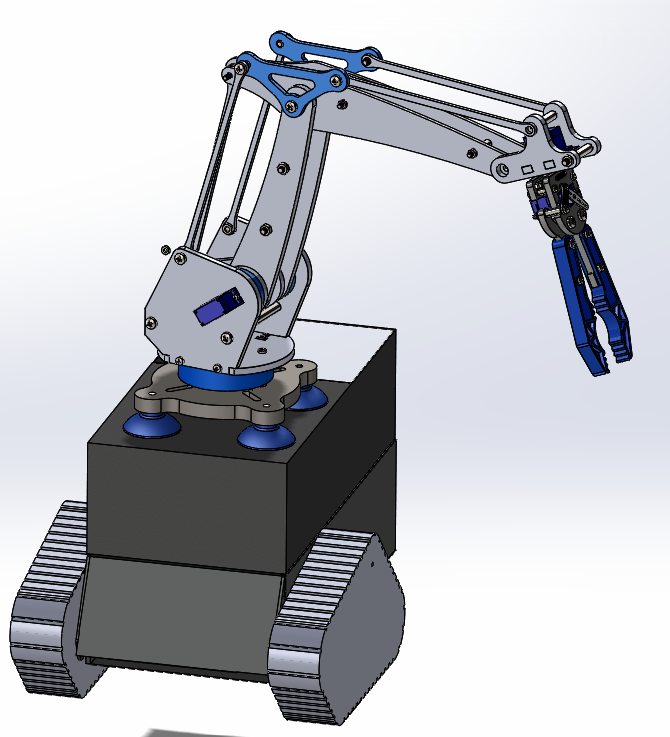
\includegraphics [width = 0.4\textwidth] {CadV2.PNG}
\caption {Grundbau des Prototypen in SolidWorks}
\end {center}
\end {figure}

\subsection {Finales Rendering des Prototypen}

\begin{figure} [ht]
\begin{center}
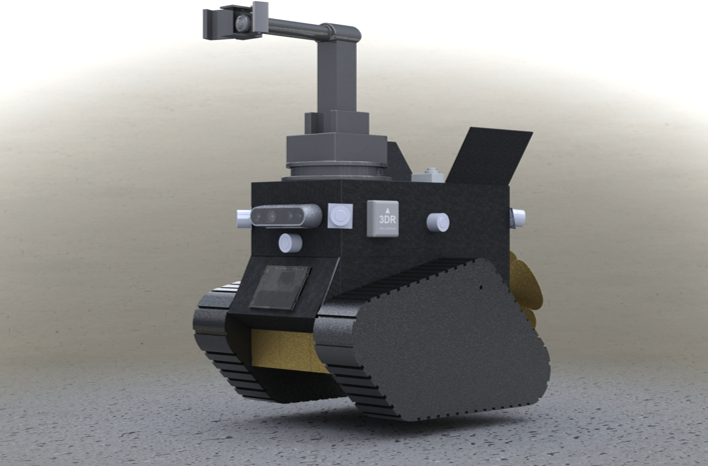
\includegraphics [width = 0.5\textwidth] {Ansicht_Vorne.PNG}
\caption {Finales Rendering des Prototypen}
\end {center}
\end {figure}

Bis hin zum fertigen Modell des Rescue Roboters und Renderings gab es viele iterative Designentscheidungen. 
Dabei wurden teils in gemeinsamen Streaming Sessions Bauteile erstellt und passend am Modell ergänzt.
Die weiteren Designentscheidungen leiteten sich aus dem Use-Case und den Requirements ab. 
Zudem erfolgte eine Hardware und Bauteil Analyse. 
Aus dieser entwickelten sich bestimmte Bauteile und Funktionen die am Roboter hinzugefügt wurden.
Dieser Entwurf des Rescue Roboters zeigt die wichtigsten Bestandteile und greift die Konzeptideen mit auf. 
Diese werden visuell und anschaulich in einem 3D-Rendering dargestellt.  Die Bauteile und Relationen bzw. Proportionen sind nicht maßstabsgetreu. 
Bis hin zur finalen Umsetzung und Realisierung des kompletten Projekts müssten diese noch verfeinert werden, um eine reale Funktion sicher und korrekt zu gewährleisten.
